\documentclass[12pt]{article}
\usepackage[utf8]{vietnam}
\usepackage[left=3.5cm, right=2cm,
top=2cm, bottom=2cm]{geometry}
\usepackage{amsmath}
\usepackage{amssymb}
\usepackage{amsthm}
\usepackage{graphicx}
% Dùng cho các tool này kia trong math 
% \adjustlimits
\usepackage{mathtools}
\usepackage{listings}
% Tạo khai báo cách mới cho Sin bằng $\Hamsin$
\DeclareMathOperator{\Hamsin}{Sin}
% Tạo ra lệnh \# thay thế cho \negmespace
\newcommand{\negmegspace}{\#}
% Tạo hàm mới với dấu phân cách
\DeclarePairedDelimiter{\tvh}{\langle}{\rangle}

\begin{document}
Tạo một hàm mới với dấu phân cách :
$$ \langle \frac{1}{2}, \frac{1}{2} \rangle $$ 
$$ \tvh{\frac{1}{2}, \frac{1}{2}} $$
Khai báo một tên hàm mới : $\Hamsin$

\vspace{1cm}

% Kí hiệu ở phía trên và ở phía dưới kí hiệu khác
% \overset{<above math>}{<math>}
$\overset{+}{B}$
$\underset{+}{B}$

\vspace{1cm}

% Mũi tên với nội dung
% $x\xleftarrow[<sub>]{<sup>}$
% $x\xrightarrow[<sub>]{<sup>}$
$\xrightarrow[<sub>]{<sup>}$
$\xleftarrow[<sub>]{<sup>}$

\vspace{1cm}

% Ngoặc ở trên hoặc dưới
$\overbrace{<math>}^{<above math>}$
$\underbrace{<math>}^{<above math>}$

% Khoảng trắng
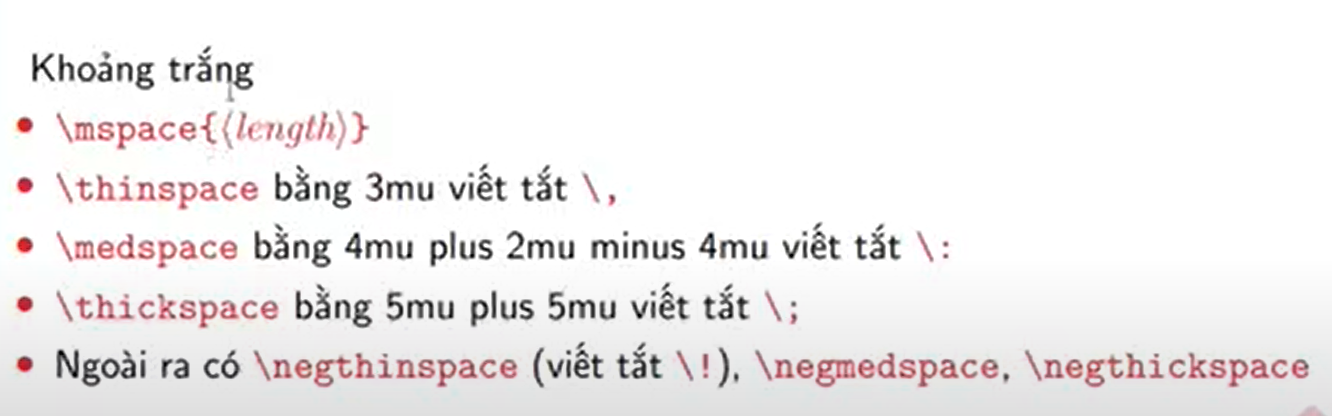
\includegraphics[scale=0.6]{image/space.png}

% Môi trường toán học
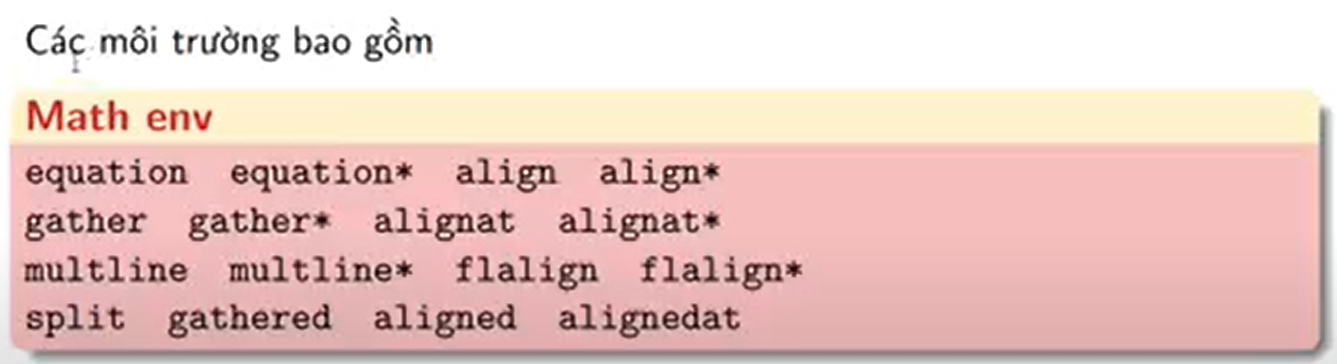
\includegraphics[scale=0.6]{image/math-environment.png}

Phương trình toán học:
\begin{equation}
	\begin{split}
    	x^2+y^2+z^2=0\\
    	xy+y^2+5=0
	\end{split}
\end{equation}

Môi trường align
\begin{align}
    x^2+y^2+z^2&=0 & xy+2+3&=0\\
    xy+y^2+5+xyz+12+6+7&=12345 & x+3y&=12 
\end{align}

Môi trường multiline:
\begin{multline}
    1231236463\\123428674\\\shoveright{12334553}\\1235432234
\end{multline}

% Tạo tag và no tag
Môi trường tag:
\begin{align}
    x^y+x_1+x_2=0 \tag*{Pt.a}\\
    x_2+x_3=0 \notag\\
    x_3+x_4=0 
\end{align}

% Chèn văn bản bằng \intertext
Chèn văn bản:
\begin{align}
    x^y+x_1+x_2&=123 \\
    x_2+x_3&=34 \\
    \intertext{Vằn bản chèn}
    x_3+x_4&=1 
\end{align}

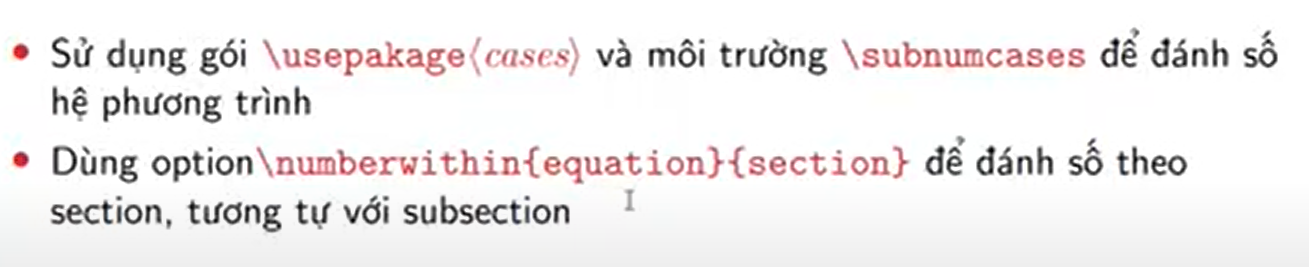
\includegraphics[scale=0.6]{image/math-environment2.png}

% code
\begin{lstlisting}[language=c++]
	#include <bits/stdc++.h>
	using namespace std;
	main()
	{
    	printf("Hello world");
	}
\end{lstlisting}
Dòng code ở trên câu lệnh \lstinline[language=python]{print "hello"}

% Math Box
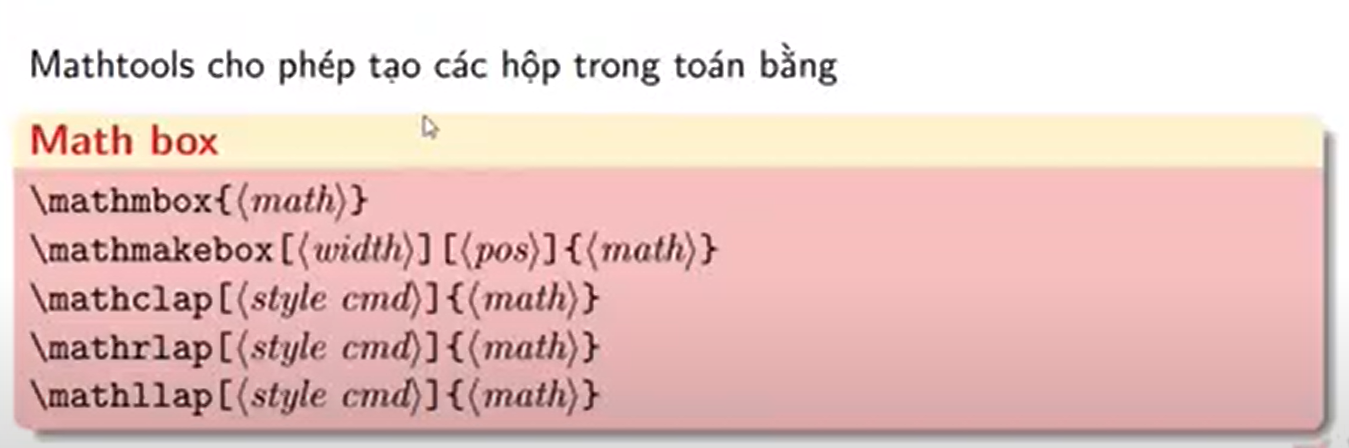
\includegraphics[scale=0.6]{image/math-box.png}\\
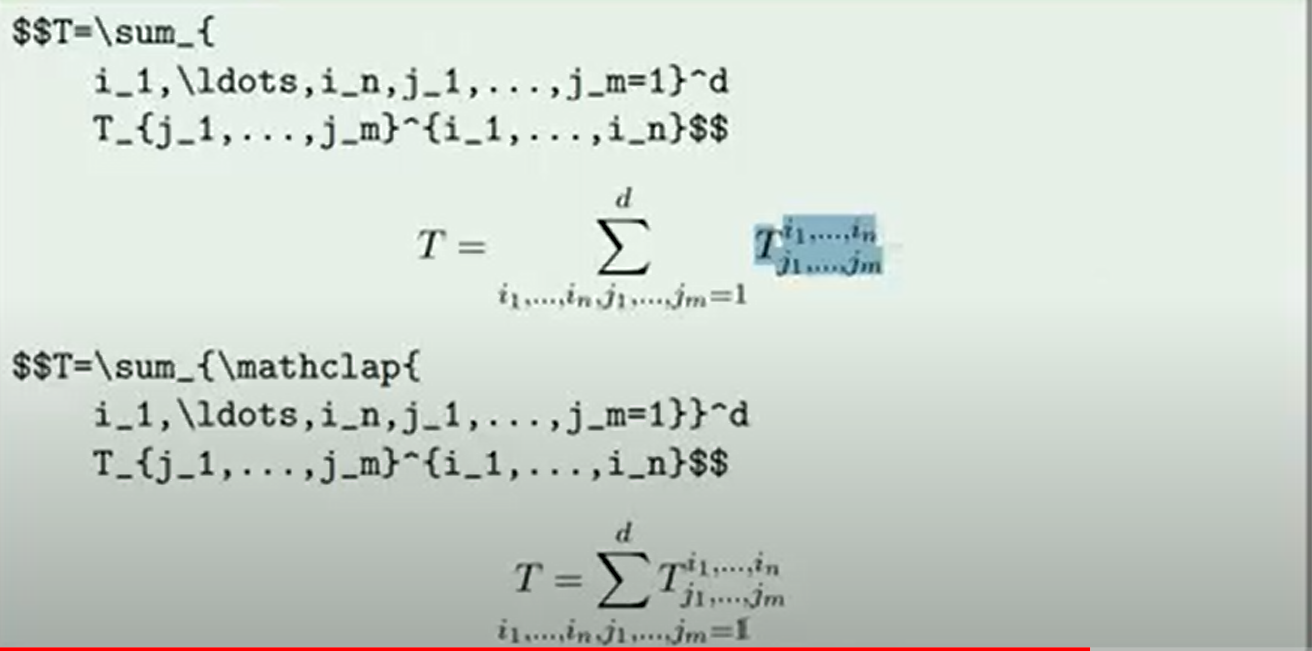
\includegraphics[scale=0.6]{image/math-box2.png}
% mathrlap chỉ một nửa cái chỉ số chạy dưới sum

\vspace{1cm}

% Adjust Limit
$\lim_{n\to\infty} \sup_{p^2\geq NK}$
\qquad
$\adjustlimits\lim_{n\to\infty} \sup_{p^2\geq NK}$

\vspace{1cm}

% Aboxed{<math>}
\begin{align*}
	\Aboxed{f(x) &= h(x)}\\
				 & = g(x)
\end{align*}

\vspace{1cm}

% Pre-script
$\prescript{14}{2}{\mathbf{C}}^{5+}_{2}$

\vspace{1cm}

%Verbatim
\begin{verbatim}
	\begin{equation}
			x + y
	\end{equation}
\end{verbatim}

\end{document}

